\section{Architecture}\label{sec:arch}

\subsection{What stays in ring 0}

The kernel is written in Rust. At the commit studied, \code{src/} holds 7,579 Rust files and 389,695 lines (our count, with \code{git ls-tree} and \code{wc}; the README says about 390,000). In 0.9.2 the same count gave 5,139 files. We have not measured where the growth sits. What we can say is what ring 0 still keeps: only address spaces and page tables, the scheduler with symmetric multiprocessing up to 256 CPUs, IPC, capabilities, the system-call boundary, process creation and the capsule spawn gate. It also keeps the TPM driver and the encrypted data volume, a hardware broker that hands device windows to driver capsules, and the kernel's record of what each Linux guest did (Section~\ref{sec:box}).\srcs{src/smp/constants.rs:17}{docs/overview/architecture-kernel-in-ring.md}

Everything else runs in ring 3. The tree has 152 directories with a \code{Capsule.mk}, up from 91 at the 0.9.2 changelog, and 67 of them are driver capsules, up from 18 (Table~\ref{tab:counts}). Figure~\ref{fig:layers} shows the split.

\begin{figure}[t]
\centering
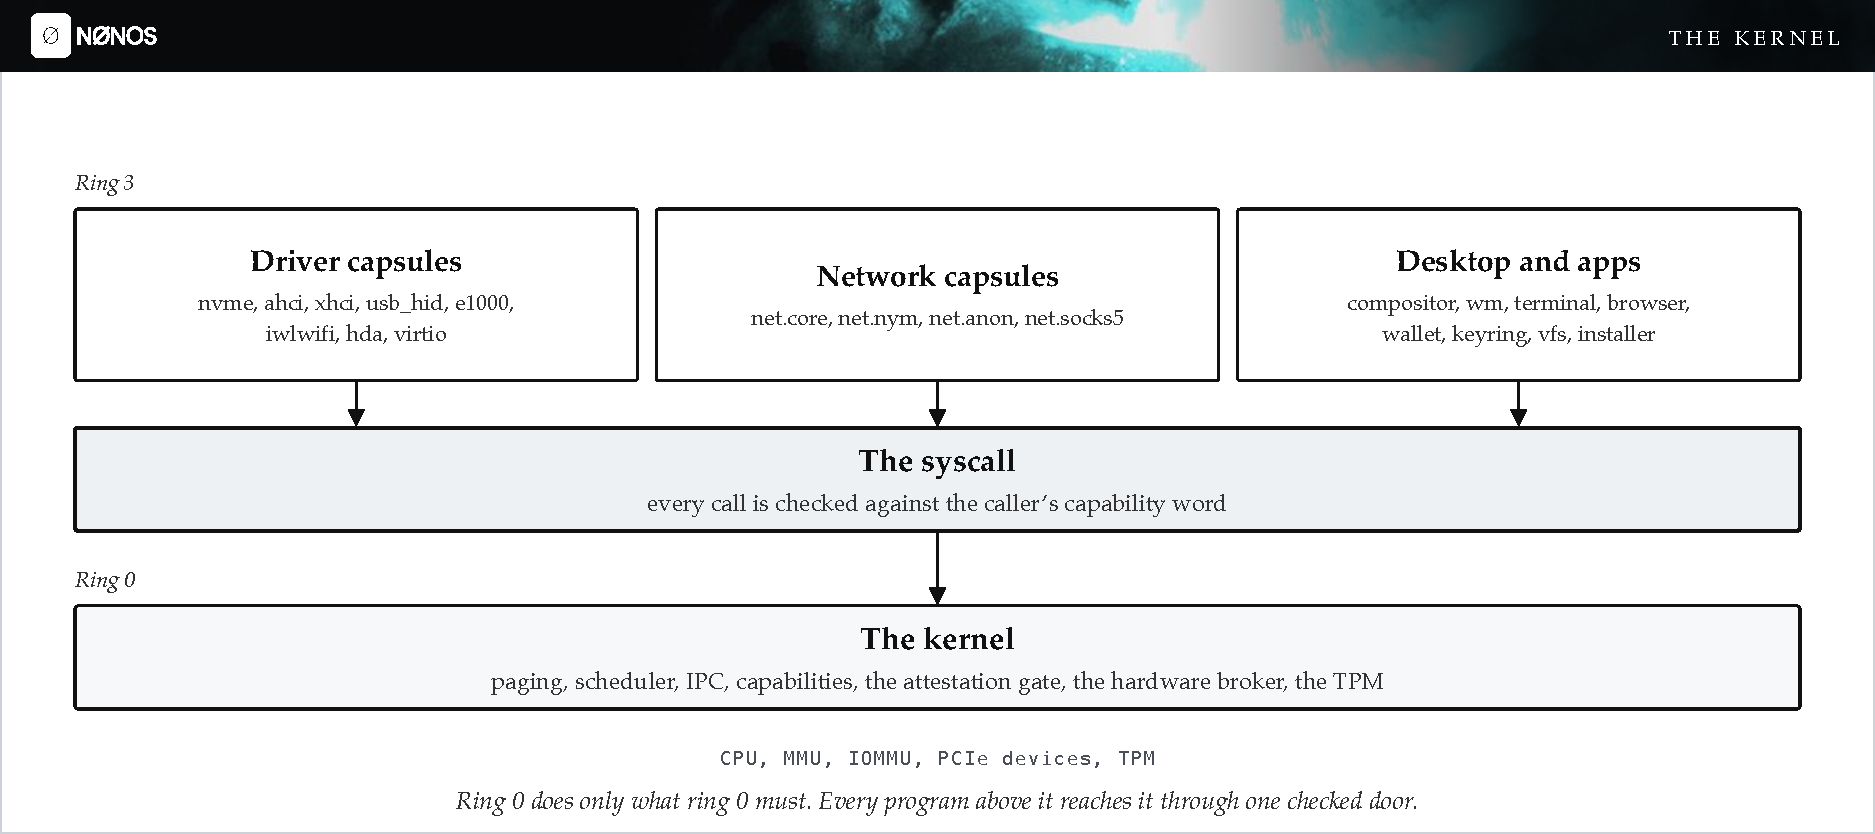
\includegraphics[width=0.84\textwidth]{figures/diagram-layers.pdf}
\caption{The kernel and everything above it. Ring 3 holds drivers, network services, the desktop and every program; ring 0 holds what only ring 0 can do. Every program reaches the kernel through one checked door, the system call. Drawn from \code{docs/overview/architecture.md} and the capsule list in the tree.}
\label{fig:layers}
\end{figure}

\begin{table}[t]
\centering
\caption{What grew between the 0.9.2 changelog and the 0.9.3 tree. Counted from git at the commit where \code{CHANGELOG-0.9.2.md} landed (6 October 2026) and at the studied commit. About 6,000 commits separate them. Capsules are directories with a \code{Capsule.mk}; proof crates are directories ending in \code{\_proofs} with a \code{Cargo.toml}.}
\label{tab:counts}
\begin{tabular}{@{}lrr@{}}
\toprule
 & 0.9.2 & 0.9.3\\ \midrule
Driver capsules & 18 & 67\\
Capsules in all & 91 & 152\\
Rust files in the kernel, \code{src/} & 5,139 & 7,579\\
Rust files in \code{userland/} & 10,069 & 31,674\\
Proof crates & 56 & 223\\
System calls & 130 & 183\\
Capability bits & 36 & 40\\ \bottomrule
\end{tabular}
\end{table}

The first four rows are the project's counts and we reproduced them from the git trees. The last two come from the ABI files, which a checker holds to the kernel.\srcs{abi/syscalls.toml}{scripts/check_syscall_abi.py} Run on this tree, the checker reports "183 published syscalls reach a handler" and \code{check\_caps\_abi.py} reports "40 published bits agree with the kernel". A word on the 0.9.2 figures: that paper counted at a later commit than the changelog, and its own count of kernel files was 5,758. We use the changelog commit for both columns so that the comparison is of like with like.

\subsection{The system-call ABI}

A call number is four ASCII letters packed into a 64-bit word. \code{MkIpcSend}, for example, is \code{MISD}. Arguments travel in \code{rdi}, \code{rsi}, \code{rdx}, \code{r10}, \code{r8} and \code{r9}. A result between $-4095$ and $-1$ is a negative errno.\srcs{abi/syscalls.toml:9-19}{src/syscall/abi/tag.rs:17-22} The kernel defines 183 calls: 167 microkernel calls, 12 cryptographic, 3 administrative and 1 for graphics. The count is the same three ways: 183 tags under \code{[numbers]} in \code{abi/syscalls.toml}, 183 variants of \code{SyscallNumber}, and a registry the checker confirms reaches a handler on every one.\srcs{abi/syscalls.toml:55-242}{src/syscall/numbers/defs.rs:6-191} The documentation page for system calls still says 176 and 147 in places; it was last counted before the latest additions, and we follow the code.\src{docs/kernel/syscalls.md}

A number the kernel does not know is the case that matters most for this release. On x86\_64 it is answered with \code{ENOSYS}, unless the caller is a Linux guest, in which case the kernel parks the guest and wakes its supervisor. A Linux system call number never collides with a \nonos{} one, because \nonos{} numbers are four letters and Linux numbers are small integers.\srcs{src/process/foreign/trap.rs:28-57}{docs/kernel/syscalls.md}

\subsection{The capability word and the check path}

Capabilities are 40 bits, defined once in \code{src/capabilities/types/defs.rs} and published in \code{abi/caps.toml}, which \code{scripts/check\_caps\_abi.py} holds to the kernel list. Bits range from \code{CoreExec} (bit 0) through \code{Network}, \code{IPC}, \code{Memory}, the device bits, to \code{DeviceSecret} (bit 35) and the four newer ones. Each process holds a token bound to its pid, its address-space id, the boot-session nonce and a revocation epoch, authenticated by a keyed BLAKE3 MAC whose key only the kernel holds.\srcs{src/process/caps.rs:38-58}{src/capabilities/token/material.rs:41-52}

Every architecture's entry hands each known call to one dispatch function, which calls \code{Capability::resolve} and returns \code{EPERM} on failure. \code{resolve} runs five checks in order: the token's MAC, expiry and revocation; the boot-session binding; the address-space binding; the revocation epoch; and whether the cap table admits this call for this word.\srcs{src/syscall/contract/dispatch.rs:31-45}{src/syscall/contract/resolver/resolve.rs:31-43} The cap table is total: a call that no table claims is refused. Figure~\ref{fig:capcheck} draws the path.

\begin{figure}[t]
\centering
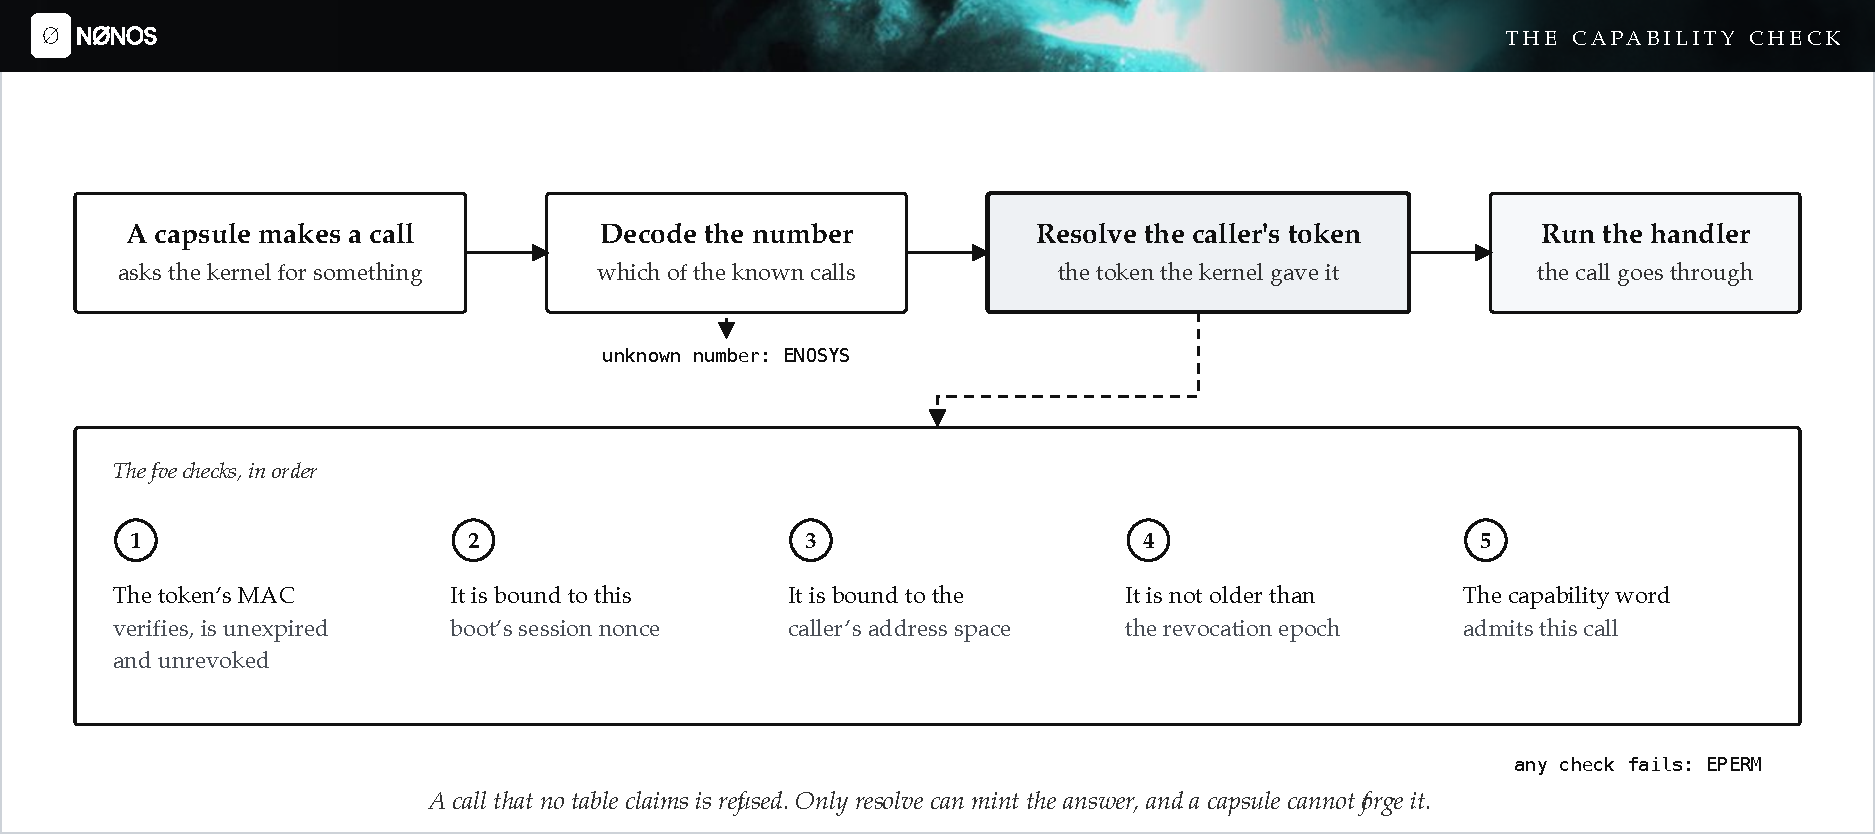
\includegraphics[width=0.84\textwidth]{figures/diagram-capability-check.pdf}
\caption{The capability check on every native system call: decode the number, resolve the caller's token, run five checks in order. Any failure is \code{EPERM}. A number that is not a native call is \code{ENOSYS}, or goes to the guest's supervisor (Section~\ref{sec:box}). Sources: \code{docs/kernel/capabilities-the-check-on.md} and \code{src/syscall/contract/resolver/resolve.rs}.}
\label{fig:capcheck}
\end{figure}

At spawn the kernel installs the word from the verified manifest exactly once. A second call is rejected, so a stale spawn path cannot reissue authority. A request for a bit the manifest does not declare is refused with \code{GrantOutsideManifest}.\srcs{src/process/caps.rs:115-127}{src/security/capsule_manifest/verify/caps.rs:31-39} A new process inherits only a small ambient set from its parent, and an air-gapped boot removes \code{Network} from every capsule.\srcs{src/process/core/table/inherit.rs:52-61}{src/kernel_core/process_spawn/capsule_spawn/runner/profile_gate.rs:48-56}

The documentation is candid about what the word does not do yet. The \code{IO} and \code{Hardware} bits gate nothing. \code{Keyring} and \code{Entropy} gate only kernel clients that no code calls. And the image-wide capability ceiling is computed and logged, not enforced: a capsule that asks for more still starts, and the log prints \code{[CEILING] not enforced, would refuse}.\srcs{docs/kernel/capabilities-what-each-bit.md}{docs/build/profiles.md}

\subsection{IPC}

Each capsule has one inbox, and a service is an endpoint in a registry with the capability bits a sender must hold. A send by name passes four gates: the \code{IPC} bit in the token; the endpoint's required bits; the held-endpoint and peer lists, which restrict who may reach a driver; and a byte budget.\src{docs/kernel/ipc-who-may-send.md} The kernel writes the sender's name itself, so a capsule cannot forge it. A payload is at most 1~MiB; all inboxes together hold at most 96~MiB, one inbox 16~MiB, and one sender at most half an inbox.\src{src/ipc/nonos_inbox/budget.rs:41-43} Reaching any of the 11 services that carry traffic off the machine takes \code{Network} as well as \code{IPC}.\src{src/services/registry/policy.rs:26-38} The peer list still has one entry: the Shield prover may send only to \code{shield.core}.\src{src/services/registry/peers.rs:27-35} Figure~\ref{fig:ipc} shows the gates.

\begin{figure}[t]
\centering
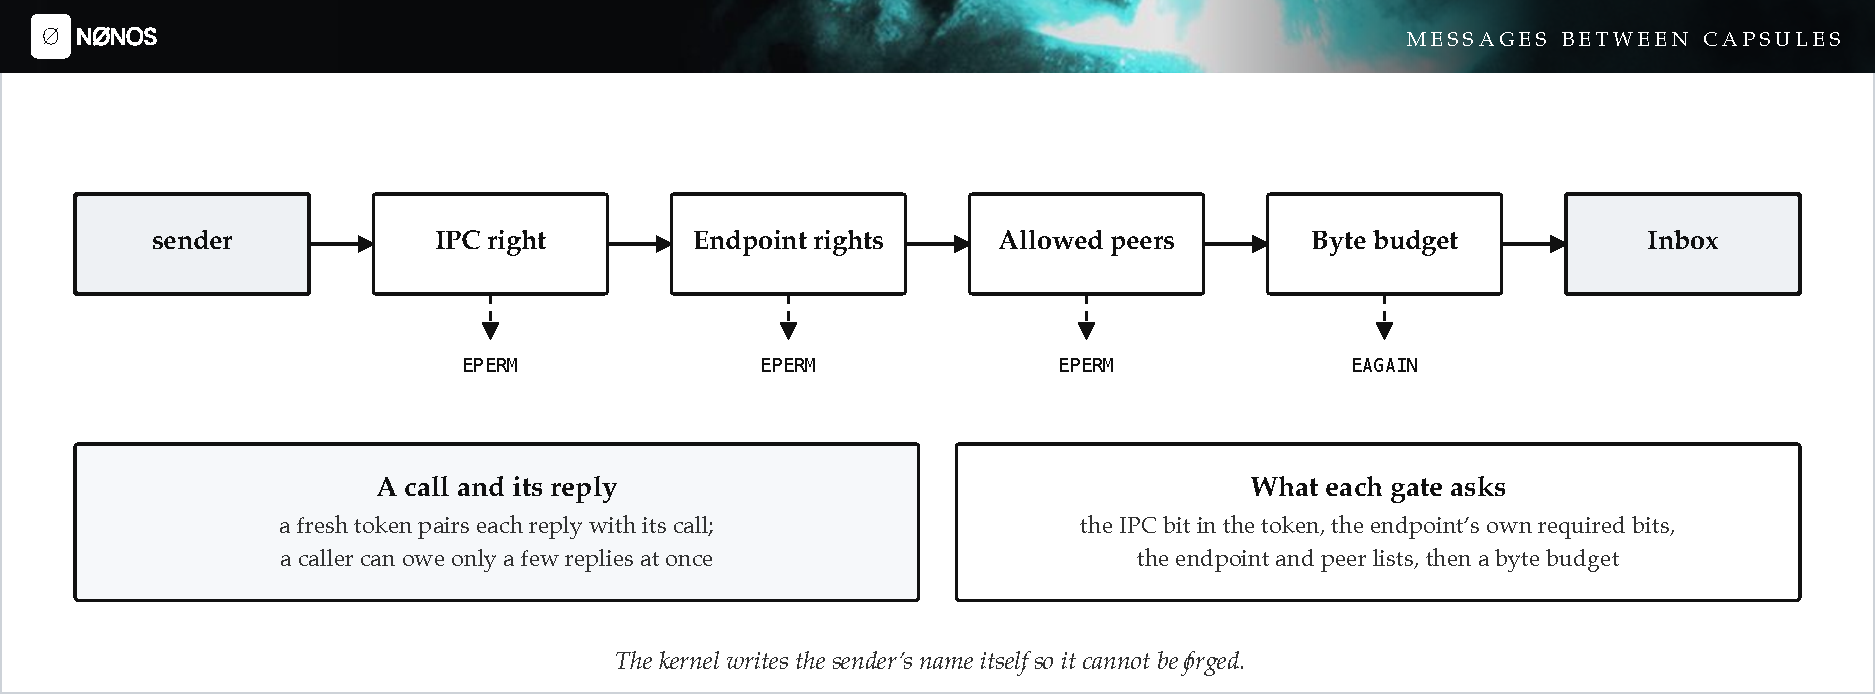
\includegraphics[width=0.84\textwidth]{figures/diagram-ipc-gates.pdf}
\caption{The four gates on a send between capsules, with the error each returns. The kernel stamps the sender's name. Sources: \code{docs/kernel/ipc-who-may-send.md}, \code{src/ipc/nonos\_inbox/budget.rs}.}
\label{fig:ipc}
\end{figure}

\subsection{Drivers and the hardware broker}

A driver capsule claims its device from the broker and then asks for MMIO windows, DMA buffers, interrupt bindings and port I/O, each behind its own capability bit. The broker gives each driver capsule its own IOMMU domain where a unit is in service, and every image turns translation on at boot. Where no unit is in service, a Standard boot goes on with the claim unconfined and says so in four places; Hardened and Air-Gapped stop.\srcs{docs/kernel/iommu-per-capsule-domains.md}{docs/release/0.9.3-security-limits.md} On release the broker stops bus mastering before it frees DMA frames.\src{docs/overview/threat-model-a-hostile-or.md}

\begin{table}[t]
\centering
\caption{The 67 driver capsules by class, generated from the \code{userland/capsule\_driver\_*} directories that hold a \code{Capsule.mk}. Which of them have run on real hardware and which only in their host model is in the hardware notes, and the answer for most is the second.}
\label{tab:drivers}
% generated by paper/tools/gen_tables.py from userland/capsule_driver_*/Capsule.mk
\begin{tabular}{@{}lr>{\raggedright\arraybackslash}p{9.2cm}@{}}
\toprule Class & Count & Drivers\\ \midrule
Storage & 12 & {\footnotesize \texttt{ahci}, \texttt{nvme}, \texttt{piix\_ide}, \texttt{buslogic}, \texttt{mpt}, \texttt{pvscsi}, \texttt{storvsc}, \texttt{ufs}, \texttt{sdhci}, \texttt{rtsx}, \texttt{virtio\_blk}, \texttt{virtio\_scsi}}\\
USB & 17 & {\footnotesize \texttt{xhci}, \texttt{ehci}, \texttt{ohci}, \texttt{uhci}, \texttt{usb\_hub}, \texttt{usb\_hid}, \texttt{usb\_msc}, \texttt{usb\_audio}, \texttt{usb\_mic}, \texttt{uvc}, \texttt{ccid}, \texttt{fido}, \texttt{cdc\_acm}, \texttt{cdc\_ecm}, \texttt{cdc\_ncm}, \texttt{rndis}, \texttt{bt\_usb}}\\
Wired network & 14 & {\footnotesize \texttt{e1000}, \texttt{e1000e}, \texttt{igb}, \texttt{igc}, \texttt{ixgbe}, \texttt{rtl8139}, \texttt{rtl8153}, \texttt{rtl8169}, \texttt{ax88179}, \texttt{pcnet}, \texttt{tulip}, \texttt{virtio\_net}, \texttt{vmxnet3}, \texttt{netvsc}}\\
Wi-Fi & 5 & {\footnotesize \texttt{iwlwifi}, \texttt{mt7921}, \texttt{rtl8821ce}, \texttt{rtl8822ce}, \texttt{rtl8852be}}\\
Input & 5 & {\footnotesize \texttt{ps2\_input}, \texttt{i2c\_hid}, \texttt{spi\_hid}, \texttt{virtio\_input}, \texttt{vmmouse}}\\
Display & 5 & {\footnotesize \texttt{bga}, \texttt{bootfb}, \texttt{intel\_display}, \texttt{virtio\_gpu}, \texttt{vmware\_svga}}\\
Audio & 2 & {\footnotesize \texttt{hda}, \texttt{ac97}}\\
Buses & 4 & {\footnotesize \texttt{gpio}, \texttt{i2c\_pci}, \texttt{spi}, \texttt{smbus}}\\
Virtual machine guests & 3 & {\footnotesize \texttt{virtio\_rng}, \texttt{vmbus}, \texttt{vmmdev}}\\
\midrule Total & 67 & \\
\bottomrule
\end{tabular}

\end{table}

\note{\path{docs/release/0.9.3-supported-hardware.md}; \path{docs/hardware/MATRIX.md}.}The 0.9.2 changelog tree had 18 driver capsules, so 49 arrived between the two trees. Each is a ring-3 process with a claim on its own device. A driver whose device is missing leaves at once, and one whose device fails gives up after a few seconds.\note{\path{README.md}, section "Drivers".} We say clearly what this does not mean. Most of the new drivers have been exercised against a model of the chip or under QEMU. On QEMU the e1000, e1000e, igb, RTL8139, PCnet, vmxnet3 and Tulip drivers each obtained a DHCP lease; the RTL8821CE has one hardware report; the other Wi-Fi drivers have run only against modelled devices.\note{\path{docs/release/0.9.3-what-is-new.md}, section "Drivers"; \path{docs/release/0.9.3-known-issues.md}, section "Hardware".}
